% Converted from Microsoft Word to LaTeX
% by Chikrii Softlab Word2TeX converter (version 5.0)
% Copyright (C) 1999-2011 Chikrii Softlab. All rights reserved.
% http://www.chikrii.com
% mailto: support@chikrii.com

% Warning: You are using Chikrii Softlab Word2TeX in TRIAL mode!
% In TRIAL mode some restrictions will apply.
% For more information please visit http://www.chikrii.com
% YOU CAN USE THIS FILE WITH THE SOLE PURPOSE OF EVALUATING Word2TeX.

\documentclass{article}
\usepackage{latexsym}
\usepackage{graphicx}
\usepackage{listingsutf8}
\usepackage{url}
\graphicspath{ {G:/TTU/Fall_17/R/Assignments/Applies/Sayan_tex} }

\begin{document}
\begin{center}
		\underline{\textbf{CS5331: ASSIGNMENT 1}}
\end{center}
	
\textbf{	rapply :}
	rapply, stands for Recursive Apply, and it is one of the more powerful function of the ‘apply’ group functions. This function is used to implement or apply a function to all elements of a list in a recursive manner. A general view of the function is as follows:
    
    $rapply(x, function()
    {<function\_definition>}, 
    class = c(“<class\_type>”), 
    how = “<how\_parameters>”)
    $
    
	The first argument is the list : x . The second argument is the function that is to be applied to the list x.
	This function has two basic modes, which are $‘how’$ and $‘classes’$. Some descriptions of the parameter ‘how’ is as follows: \leavevmode\newline
	
	\begin{itemize}
	 \item	how = “replace” : The elements in the list which itself is not a list, and has a class included in ‘classes’ is replaced by the result, generated by applying the function to the elements.
	 
	\item how = “list” : All non-list elements whose class is included in ‘classes’ are replaced by the result, generated by applying the function to the elements. All other elements are replaced by the default result.
	
    \end{itemize}
	
	After implementing a comparative code between rapply() and its equivalent loop, benchmark was measured, and the performance was plotted. The code is as follows : \\
\lstset{language=R}


\begin{lstlisting}
	
library("microbenchmark")
#Creating a demo list
demo_list <- list(1:5,list(6:9),10:12,list(13:20))

#Applying rapply to find squares of each element
rapply_function <- function()
{
list_rapply <- rapply(demo_list, function(demo_list){demo_list^2})
}

#Using loops to do the same evaluations

list_loop<- list()
loop_function <- function()
{
for(i in 1:length(demo_list))
{
for(j in 1:length(demo_list[[i]]))
{
if(class(demo_list[[i]][j]) == "list")
{
subList <- demo_list[[i]][j]
for(k in 1:length(subList[[1]]))
list_loop <- c(list_loop,subList[[1]][k]^2)
}
else
{
list_loop <- c(list_loop,demo_list[[i]][j]^2)
}
}
}
}

#Benchmarking both the functions
microbenchmark(rapply_function(),loop_function())

# Performance graph for rapply
performance_rapply <- data.frame(Replications = 
character(), Elapsed_Time = numeric())
rep <- c(100,500,1000,1500,2000)
for(i in rep){
tmp <- benchmark(rapply(demo_list, 
function(demo_list){demo_list^2}))
performance_rapply <- rbind(performance_rapply, 
data.frame(as.character(i), tmp))
}
names(performance_rapply) <- c("replications",
"elapsed_time")

# Performance graph for loop
performance_for <- data.frame(Replications = 
character(), Elapsed_Time = numeric())
rep <- c(100,500,1000,1500,2000)
for(i in rep){
tmp <- benchmark(loop_function(), replications = i)
performance_for <- rbind(performance_for, 
data.frame(as.character(i), tmp))
}
names(performance_for) <- c("replications","loop_time")

performance_final <- cbind(performance_rapply, 
performance_for$loop_time)
names(performance_final) <- "loop_time"


#plot for the performance comparison
ggplot(performance_final, aes(x = as.integer(replications))) + 
geom_line(aes(y = elapsed_time, colour = "rapply_time")) + 
geom_line(aes(y = loop_time, colour = "loop_time"))


	
\end{lstlisting}
	Benchmark was taken for 10 instances, they are as follows:
	\begin{center}
		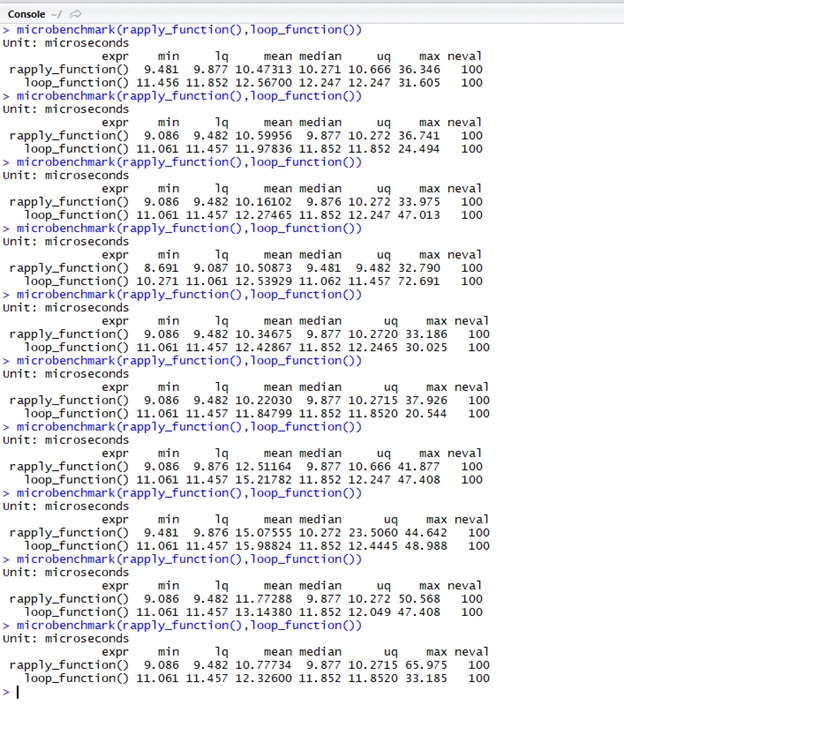
\includegraphics{benchmark_rapply.jpg}	
	\end{center}

	

	A graph was plotted for 5 instances, and the result found are as follows:
	
	\begin{center}
		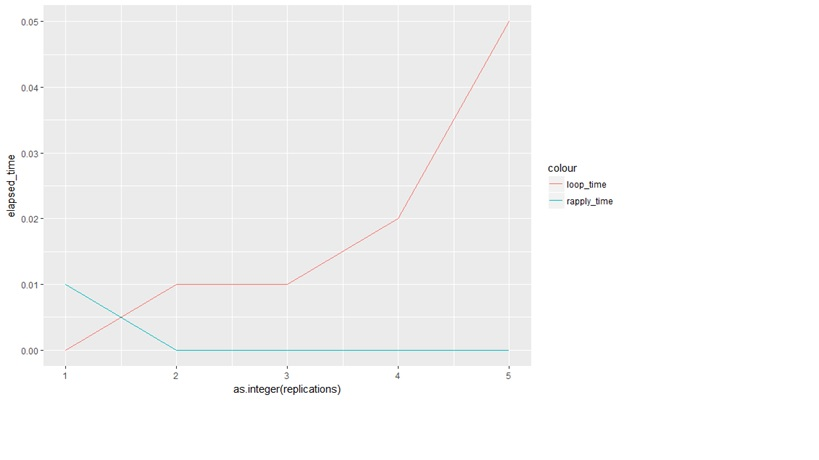
\includegraphics{plot_rapply.jpg}
	\end{center}
	
	From the results, we can see, that rapply, performs the same task in a better time. This can be seen by observing the mean values of both the functions for the benchmarks, and from the graph plotted.
    \pagebreak
	
	\textbf{tapply} :
	A Ragged array in R, is an array containing values given by a unique combination of the levels of certain factors. tapply applies a function to each cell of a ragged array. A general view of the function is as follows:
	
	$$tapply(x, INDEX, function(){<function\_definition>}, default = NA, simplify = TRUE)$$
	The description of the arguments are as follows:\leavevmode\newline
	
	\begin{itemize}
	\item	x : An R object for which a split method exists.
	\item	INDEX : a list of one or more factors having the same length as x.
	\item	function : the function that is to be applied to the list.
	\item	default : the value with which the array is initialized as array. Only in case of simplification to an array.
	\item	simplify : if FALSE, tapply will always return an array mode “list”. If TRUE, then the function always returns an array with the mode of scalar.
	
\end{itemize}
	After implementing a comparative code between tapply() and its equivalent loop, benchmark was measured, and the performance was plotted. The code is as follows :
	
	\lstset{language=R}
	
	\begin{lstlisting}
	
library(microbenchmark)
library(ggplot2)

# Creating a demo data_frame, assigning student_id and
 randoming marks, and adding labels, based on year
df_demo <- data.frame(student_id = 1:10000,
 marks =rnorm(10000, mean = 60, sd = 10),
year = gl(4, 2500,
labels = c("2017","2016","2015","2014")))

#Assigning grades according to marks obtained
for(i in seq_along(df_demo$student_id))
{
if(df_demo$marks[i] > 90)
{
df_demo$grade[i] <- "O"
}
else if(df_demo$marks[i] > 80)
{
df_demo$grade[i] <- "E"
}
else if(df_demo$marks[i] > 75)
{
df_demo$grade[i] <- "A"
}
else if(df_demo$marks[i] > 70)
{
df_demo$grade[i] <- "B"
}
else if(df_demo$marks[i] > 65)
{
df_demo$grade[i] <- "C"
}
else if(df_demo$marks[i] > 60)
{
df_demo$grade[i] <- "D"
}
else
{
df_demo$grade[i] <- "F"
}
}

#Using tapply to find mean of marks based on year
tapply_function <- function()
{
tapply(df_demo$marks, df_demo$year, mean)
}

#Using loop to find the same
loop_function <- function()
{
for(i in unique(df_demo$year))
{
c(mean(df_demo[which(df_demo$year == i),"marks"]),i)
}
}
loop_function()
tapply_function()

#benchmarking
microbenchmark(tapply_function(),loop_function())

# Performance graph for tapply
performance_tapply <- data.frame(Replications = character(),
 Elapsed_Time = numeric())
rep <- c(100,500,1000,1500,2000)
for(i in rep)
{
tmp <- benchmark(tapply(df_demo$marks, df_demo$year, mean))
performance_tapply <- rbind(performance_tapply,
 data.frame(as.character(i), tmp))
}
names(performance_tapply) <- c("replications","elapsed_time")

# Performance graph for loop
performance_for <- data.frame(Replications = character(),
 Elapsed_Time = numeric())
rep <- c(100,500,1000,1500,2000)
for(i in rep)
{
tmp <- benchmark(loop_function(), replications = i)
performance_for <- rbind(performance_for, data.frame(as.character(i), tmp))
}
names(performance_for) <- c("replications","elapsed_time_for")

performance_final <- cbind(performance_tapply,
 performance_for$elapsed_time_for)
names(performance_final) <- "elapsed_time_for"


#plot for the performance comparison
ggplot(performance_final, aes(x = as.integer(replications))) + 
geom_line(aes(y = elapsed_time, colour = "tapply_time")) + 
geom_line(aes(y = elapsed_time_for, colour = "loop_time"))


\end{lstlisting}
	The benchmark for 10 instances are as follows :
\begin{center}
	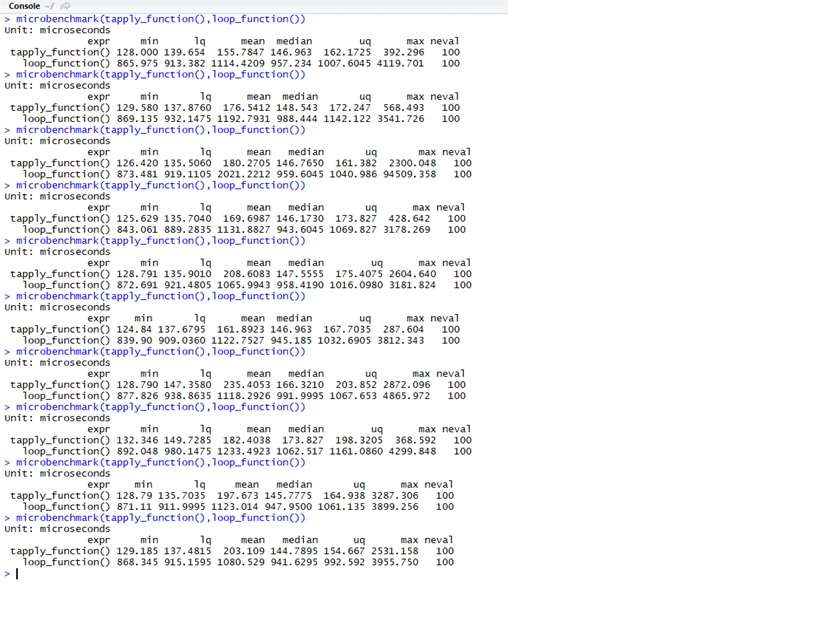
\includegraphics{benchmark_tapply.jpg}
\end{center}

\pagebreak
A graph was plotted for 5 instances, and the result found are as follows:

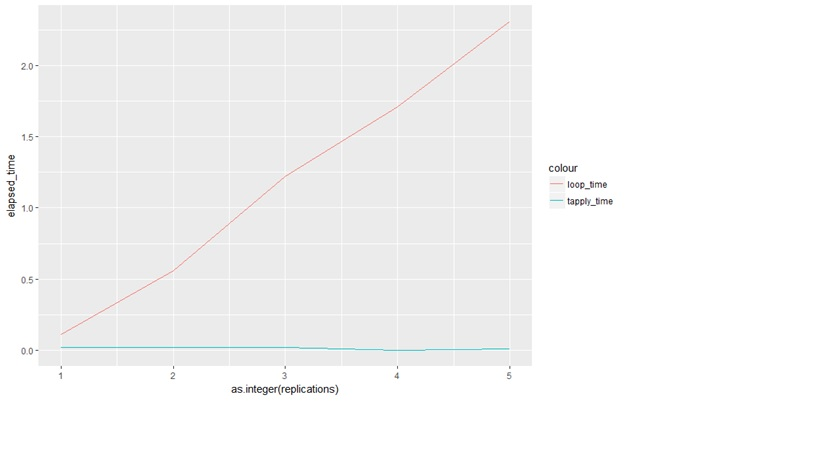
\includegraphics{plot_tapply.jpg}
From the results, we can see, that tapply, performs the same task in a better time. This can be seen by observing the mean values of both the functions for the benchmarks, and from the graph plotted.

\pagebreak

\textbf{mapply :}
This apply function is a multivariate version of sapply. mapply applies a function to the first elements of each argument, the second elements, the third elements, and so on. The arguments are recycled if necessary. A general view of the function is as follows: 

$mapply(function(){<function definition>}, ..., MoreArgs = NULL, SIMPLIFY = TRUE, USE>NAMES = TRUE
)$

The description of the arguments are as follows: \leavevmode\newline
\begin{itemize}
	\item	function : function that is to be applied
	\item	... : arguments to vectorize over.
	\item	MoreArgs : a list of other arguments to the function.
	\item	SIMPLIFY : logical or character string.
	\item	USE.NAMES : logical values as input. If the first … argument has names, or if it is a character vector, the character vector is used as the names.
\end{itemize}
After implementing a comparative code between mapply() and its equivalent loop, benchmark was measured, and the performance was plotted. The code is as follows :

\lstset{language=R}

\begin{lstlisting}

library(microbenchmark)
library(ggplot2)

#using mapply to find sum of respective elements of sub_1, sub_2 and sub_3
demo_list <- list(sub_1 = c(1:10), sub_2 = c(11:20), sub_3 = c(21:30))
mapply_function <- function()
{
results_mapply <- mapply(sum, demo_list$sub_1, 
demo_list$sub_2, demo_list$sub_3)
}


#Equivalent for loop
loop_function <- function()
{
temp <- 1
results_loop <- list()
for(i in 1:length(demo_list[[temp]]))
{
results_loop<- c(results_loop,(demo_list$sub_1[i] +
 demo_list$sub_2[i] + demo_list$sub_3[i]))
}
}
loop_function()

microbenchmark(mapply_function(),loop_function())


# Performance graph for mapply
performance_mapply <- data.frame(Replications = character(),
Elapsed_Time = numeric())
rep <- c(100,500,1000,1500,2000)
for(i in rep)
{
tmp <- benchmark(mapply(sum, demo_list$sub_1, demo_list$sub_2,
demo_list$sub_3))
performance_mapply <- rbind(performance_mapply,
 data.frame(as.character(i), tmp))
}
names(performance_mapply) <- c("replications","elapsed_time")

# Performance graph for loop
performance_for <- data.frame(Replications = character(),
 Elapsed_Time = numeric())
rep <- c(100,500,1000,1500,2000)
for(i in rep)
{
tmp <- benchmark(loop_function(), replications = i)
performance_for <- rbind(performance_for, data.frame(as.character(i), tmp))
}
names(performance_for) <- c("replications","elapsed_time_for")

performance_final <- cbind(performance_mapply,
 performance_for$elapsed_time_for)
names(performance_final) <- "elapsed_time_for"


#plot for the performance comparison
ggplot(performance_final, aes(x = as.integer(replications))) + 
geom_line(aes(y = elapsed_time, colour = "mapply_time")) + 
geom_line(aes(y = elapsed_time_for, colour = "loop_time"))	

	
	\end{lstlisting}
	The benchmark for 10 instances are as follows :
	\begin{center}
		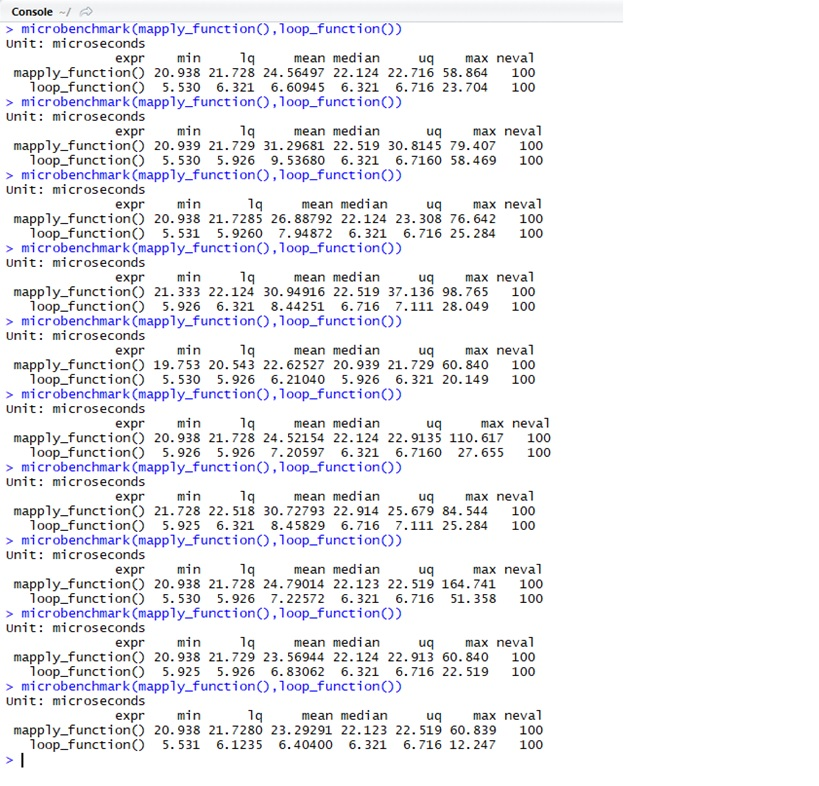
\includegraphics{benchmark_mapply.jpg}
	\end{center}
	
 
   A graph was plotted for 5 instances, and the result found are as follows:
   
    \begin{center}
    	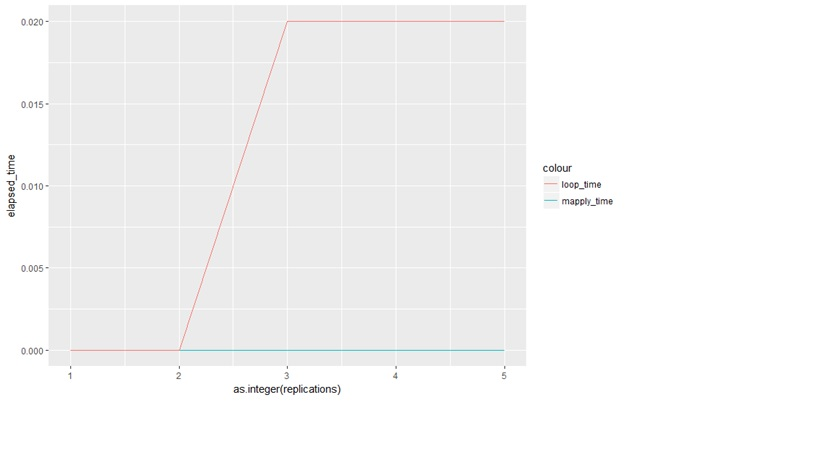
\includegraphics{plot_mapply.jpg}
    \end{center}
    From the results, we can see, that mapply, performs the same task in a better time. This can be seen by observing the mean values of both the functions for the benchmarks, and from the graph plotted.
    \linebreak
    
    \underline{\textbf{REFERENCE}}
    \linebreak
	\url{https://github.com/sm2k2010/R_Fall17_Assignments}
\end{document}
